For a generic field transformation, we can take inspiration from an MD update, where
\begin{equation}
	U' ← U \exp[\dd t \ProjTAH(M)].
\end{equation}
$U$ is covariant and $M$ (being sum of loops) is invariant under gauge transformation.

The most generic form of a field transformation could be
\begin{equation}
	U(x,μ)' ← \ProjSU \sum_L a_L \OrdProd[L(x,μ)],
\end{equation}
where $L(x,μ)$ is any line connecting gauge links from $x$ to $x+\hat{μ}$, $a_L$ is a scalar coefficient.
$L(x,μ)$ may or may not need to go through $U(x,μ)$.
wet may also have loops in it, and results in a polynomial of such loop after sum.

The $\ProjSU$ has to satisfy the constraint that
\begin{equation}
	X \ProjSU(M) Y = \ProjSU(X M Y)
\end{equation}
for any $X$ and $Y$ in the group.

We can, however, rewrite the equation to be similar to the MD update,
\begin{equation}
	U(x,μ)' ← \ProjSU \sum_L a_L U(x,μ) U(x,μ)^\dag \OrdProd[L(x,μ)],
\end{equation}
such that
\begin{equation}
	U(x,μ)^\dag \OrdProd[L(x,μ)]
\end{equation}
becomes a complete loop, which is gauge invariant.
We then have it in a simplified form,
\begin{equation}
	U' ← \ProjSU \sum_R a_R U R,
\end{equation}
where $R$ is any loop that start and stop at $x+\hat{μ}$.

We may write it in terms of
\begin{equation}
	U' ← \ProjSU \sum_{LR} a_{LR} L U R,
\end{equation}
such that L is any loop that start and stop at $x$, but since we can always pull the $U$ to the left by multiplying $U U^\dag$, the most generic form is simply,
\begin{equation}
	U' ← \ProjSU[ U (\sum_R a_R R) ],
\end{equation}
where $R$ is any loop that start and stop at $x+\hat{μ}$, and may or may not go through $U$.

We can multiply $U U^\dag$ again, so it becomes
\begin{equation}
	U' ← U { U^\dag \ProjSU[ U (\sum_R a_R R) ] }.
\end{equation}
If we had a $\ProjSU$ that satisfies
\begin{equation}
	X \ProjSU(M) Y = \ProjSU(X M Y)
\end{equation}
the above update would become
\begin{equation}
	U' ← U \ProjSU[ \sum_R a_R R ]
\end{equation}
though we need $\ProjSU$ satisfy a different constraint,
\begin{equation}
	X \ProjSU(M) X^\dag = \ProjSU(X M X^\dag)
\end{equation}
If we were allowed to do the above change of constraint to $\ProjSU$, it seems we could just use the projection in MD update,
\begin{equation}
	U' ← U \exp[ \ProjTAH( \sum_R a_R R ) ]
\end{equation}

It looks like we are only one step away from
\begin{equation}
	U' ← U \exp\left[ \frac{\dd}{\dd U} \F( \ReTr A, \ReTr B, \ReTr C, ... ) \right]
\end{equation}
where $\F$ is any analytical function or neural network, and $A$, $B$, $C$, ... are any closed
loops may or may not passing $U$.

We can simplify it by moving the $U$ independent loops out and keeping
the $U$ dependent loops simple,
\begin{equation}
\label{eq:gen-smear}
	U' ← U \exp\left[ c \atan\left[\F(\ReTr X, \ReTr Y, ...)\right] \left[\frac{\dd}{\dd U} \ReTr[W]\right] \right]
\end{equation}
so that $\F(\ReTr X, \ReTr Y, ...)$ only depends on $U$ independent loops,
while $W$ contains $U$ dependent loops, $c \atan(\F)$ is for restricting
the Jacobian to be positive definite, and $W$ is a sum of any loop
and its symmetrized versions including $U$.
The arbitrary function $\F$ can take the form of a neural network.

For a transformation to be usable in HMC, we want a tractable Jacobian determinant.
One way to achieve this is updating gauge links in subsets,
such that each update to the subset of $U$ has a Jacobian matrix,
where the only nonzero entries are on its diagonal.

\begin{figure}
	\centering
	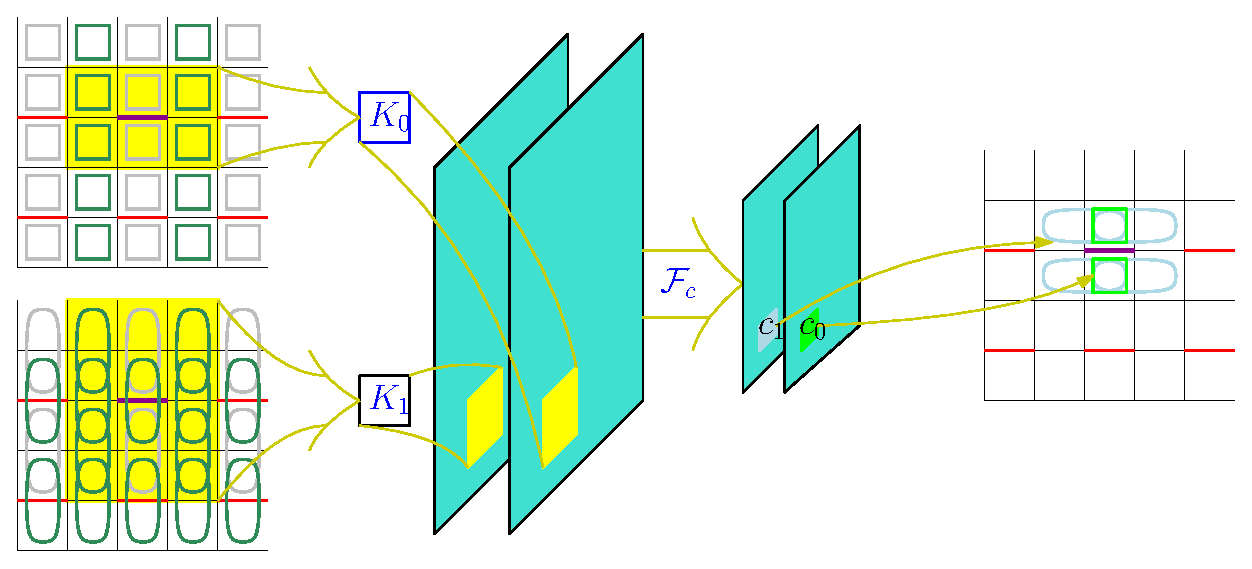
\includegraphics[width=\textwidth]{filters.eps}
	\caption{\label{fig:filters}Example generic filters for gauge covariant update of selected links.  See text for details.}
\end{figure}

Figure~\ref{fig:filters} shows an example of generic field transformation.
We identify the subset of the gauge links to update in red, computing the
gauge invariant Wilson loops, and mask out those loops depending on the
to-be-updated links.
We apply convolutional neural networks, with kernels $K_0$ for the plaquettes
and $K_1$ for the rectangles, applying to the green unmasked Wilson loops,
with their respective kernel sizes in yellow.
We then stack the results of the previous networks together and apply further
convolutional neural network $\F_c$ to it as a whole.
The result of this neural network provides the coefficients, $c_0$ and $c_1$,
for the local update depending on the plaquette and rectangle terms respectively.
